\chapter{Reason: Driving with Graph Visual Question Answering}\label{ch:drivelm}
\begin{contribution}
This chapter is based on the ECCV 2024 paper ``DriveLM: Driving with Graph Visual Question Answering''~\cite{sima2024drivelm}, of which the author is a co-first author with Katrin Renz; Andreas Geiger and Hongyang Li are the project leads. The author proposed the Graph VQA task and its graph structure, from perception through prediction and planning to behaviour and motion; designed and built DriveLM-nuScenes, including the question templates, the annotation pipeline and the management of human annotation; designed and implemented the DriveLM-Agent baseline; conducted the experiments and analyses on nuScenes and Waymo; designed the evaluation metrics; wrote the paper; and was the lead organiser of the ``Driving with Language'' track of the CVPR 2024 Autonomous Grand Challenge. DriveLM-CARLA and the CARLA generalisation experiments were led by co-authors, and the PDM-Lite expert used to generate DriveLM-CARLA was developed by Jens Bei{\ss}wenger~\cite{beisswenger2024pdmlite}. Material from~\cite{sima2024drivelm} is reproduced with permission from Springer Nature (Computer Vision -- ECCV 2024, Lecture Notes in Computer Science, vol.~15110, pp.~256--274).
\end{contribution}

Chapter~\ref{ch:occnet} gave the agent a general description of what is where. Such a description is necessary, but it does not tell the agent what to do. A driver who knows where every object is must still decide which objects matter, how they are likely to move and how to respond. When the situation is one that training never covered, such as an unfamiliar sensor configuration or a road user of a kind never seen before, these decisions cannot be read off from past examples; they have to be reasoned out. Reasoning is therefore the second front on which a physical agent meets the curse of reality.

Vision-language models (VLMs) trained on web-scale data are an obvious source of such reasoning. They carry broad knowledge of the world, they communicate in language that people can read and question, and they can break a decision into several logically connected steps. They are not, however, grounded in driving. A general VLM has never been asked to turn a camera image into a trajectory, and the driving question-answering datasets available when this work began asked either one scene-level question or a short chain of questions about a single object. Neither format reflects how human drivers reason: they consider several objects and reason about each of them in several steps, from perception through prediction to planning. This gap leads to the second research question of the thesis:
\begin{quote}
\textbf{RQ2 (Reason).} \emph{How can the general knowledge of vision-language models be grounded in driving through structured, human-inspectable steps from perception through prediction to planning, and does such reasoning help a driving agent generalise to unseen situations?}
\end{quote}

This chapter answers RQ2 with DriveLM: a task, two datasets, metrics and a VLM baseline for driving with language. Graph VQA links perception, prediction, planning, behaviour and motion QAs in a directed acyclic graph. DriveLM-nuScenes contains 4,871 frames with 91.4 QAs per frame on average; DriveLM-CARLA contains about 1.6 million template-generated QAs collected with PDM-Lite~\cite{beisswenger2024pdmlite}. DriveLM-Agent passes parent answers to child questions as context and represents trajectories as tokens. In-domain, graph context does not improve its open-loop planning result. On Waymo, most of the displayed advantage over single-frame UniAD comes from the pre-trained backbone: ADE is 2.63 with graph context, 2.76 without context and 2.78 for the motion-only BLIP-2 baseline, against 4.16 for UniAD-Single; speed accuracy is 54.29 with graph context and 43.90 without it. In CARLA, adding a pedestrian-specific question raises behaviour accuracy on selected pedestrian scenes from 4.59 to 27.04 while lowering regular-scene accuracy from 59.63 to 52.17. These are single-run associations under different context conditions, not an isolated causal effect of graph topology.

Section~\ref{drivelm:sec:motivation} develops the motivation and Section~\ref{drivelm:sec:related} reviews related work. Section~\ref{drivelm:sec:gvqa} formulates GVQA and its metrics, Section~\ref{drivelm:sec:data} describes DriveLM-Data, and Section~\ref{drivelm:sec:agent} introduces DriveLM-Agent. Section~\ref{drivelm:sec:experiments} reports the experiments and Section~\ref{drivelm:sec:discussion} discusses their limitations. Section~\ref{drivelm:sec:community} describes how the benchmark was taken up and audited by the community, and Section~\ref{drivelm:sec:summary} summarises the chapter. Further details are collected in Appendix~\ref{app:drivelm}.

\section{Motivation}\label{drivelm:sec:motivation}

Current autonomous driving stacks still lack crucial capabilities~\cite{chen2024e2esurvey,chib2023recent}. The first is generalisation: the ability to handle unseen scenarios or unfamiliar sensor configurations. The second is transparent interaction with humans, which is relevant to broader regulatory discussions of explanation and accountability~\cite{atakishiyev2023explaining}. Moreover, today's driving models plan on geometrically precise bird's-eye-view (BEV) representations~\cite{hu2023uniad,chitta2023transfuser,li2023bevdevils}, whereas humans do not. Humans implicitly perform object-centric perception, prediction and planning, which we refer to as $P_{1-3}$: a rough identification and localisation of the key objects, followed by reasoning about their possible movement and the aggregation of this information into a driving action~\cite{Marr82,spelke2007core}.

VLMs~\cite{li2023blip2,zhang2023llamaadapter,liu2023llava,wang2023visionllm} have three strengths that match these needs. First, they hold a base understanding of the world, learned from internet-scale data, that could facilitate generalisation in planning; VLMs have already achieved this kind of generalisation in simpler robotics tasks~\cite{zitkovich2023rt2,driess2023palme}. Second, language as input and output offers a platform for human-friendly interaction, unlike the bounding boxes or trajectories that are more common in current methods~\cite{li2022bevformer,hu2022stp3,Renz2022CORL,dauner2023parting}. Third, VLMs can express decisions in multiple linked steps~\cite{zitkovich2023rt2,wei2022cot,wang2023selfconsistency,yao2023tree,besta2023got,ding2023everything}. The individual VLM calls remain differentiable during fine-tuning, but the complete multi-stage inference pipeline passes discrete text between separately adapted stages and is not trained jointly end to end.

At the time of this work, efforts to apply VLMs to driving relied on two kinds of visual question answering (VQA). Scene-level VQA describes the driving behaviour with one or two supporting reasons, \eg, ``The car is moving into the right lane because it is safe to do so''~\cite{kim2018bddx,kim2019had}. Single object-level VQA explains the response of the ego vehicle to one object through a chain of questions of the form ``what--which--where--how--why'', \eg, ``The ego vehicle stops because there is a pedestrian in a white shirt crossing the intersection in front of the ego vehicle and it does not want to crash into the pedestrian''~\cite{sachdeva2023rank2tell,malla2023drama,qian2024nuscenesqa}. Neither paradigm is a suitable proxy for the $P_{1-3}$ reasoning of human drivers, who consider multiple objects and reason about each of them in multiple steps.

DriveLM therefore changes the proxy task rather than the model (Fig.~\ref{drivelm:fig:teaser}). In GVQA, the questions of a frame are linked by logical dependencies that can guide the answering process, and the chain of questions ends with the behaviour and motion of the ego vehicle, so that answering the graph amounts to driving. Two design choices follow from the aim of generalisation. First, the training data are paired with test settings that demand zero-shot generalisation: a new sensor configuration (training on nuScenes~\cite{caesar2020nuscenes} and testing on Waymo~\cite{sun2020waymo}) and a new object class (pedestrians, which never appear in the training data of DriveLM-CARLA). Second, the contribution lies in the task, the data, the metrics and an official evaluation server rather than in a new algorithm. The young field of driving with language lacked a standardised dataset, task and evaluation framework, so we make no claim of algorithmic novelty and keep the baseline intentionally simple. This follows the benchmark-driven research cycle described in Chapter~\ref{ch:methodology}.

\begin{figure}[t]
  \centering
  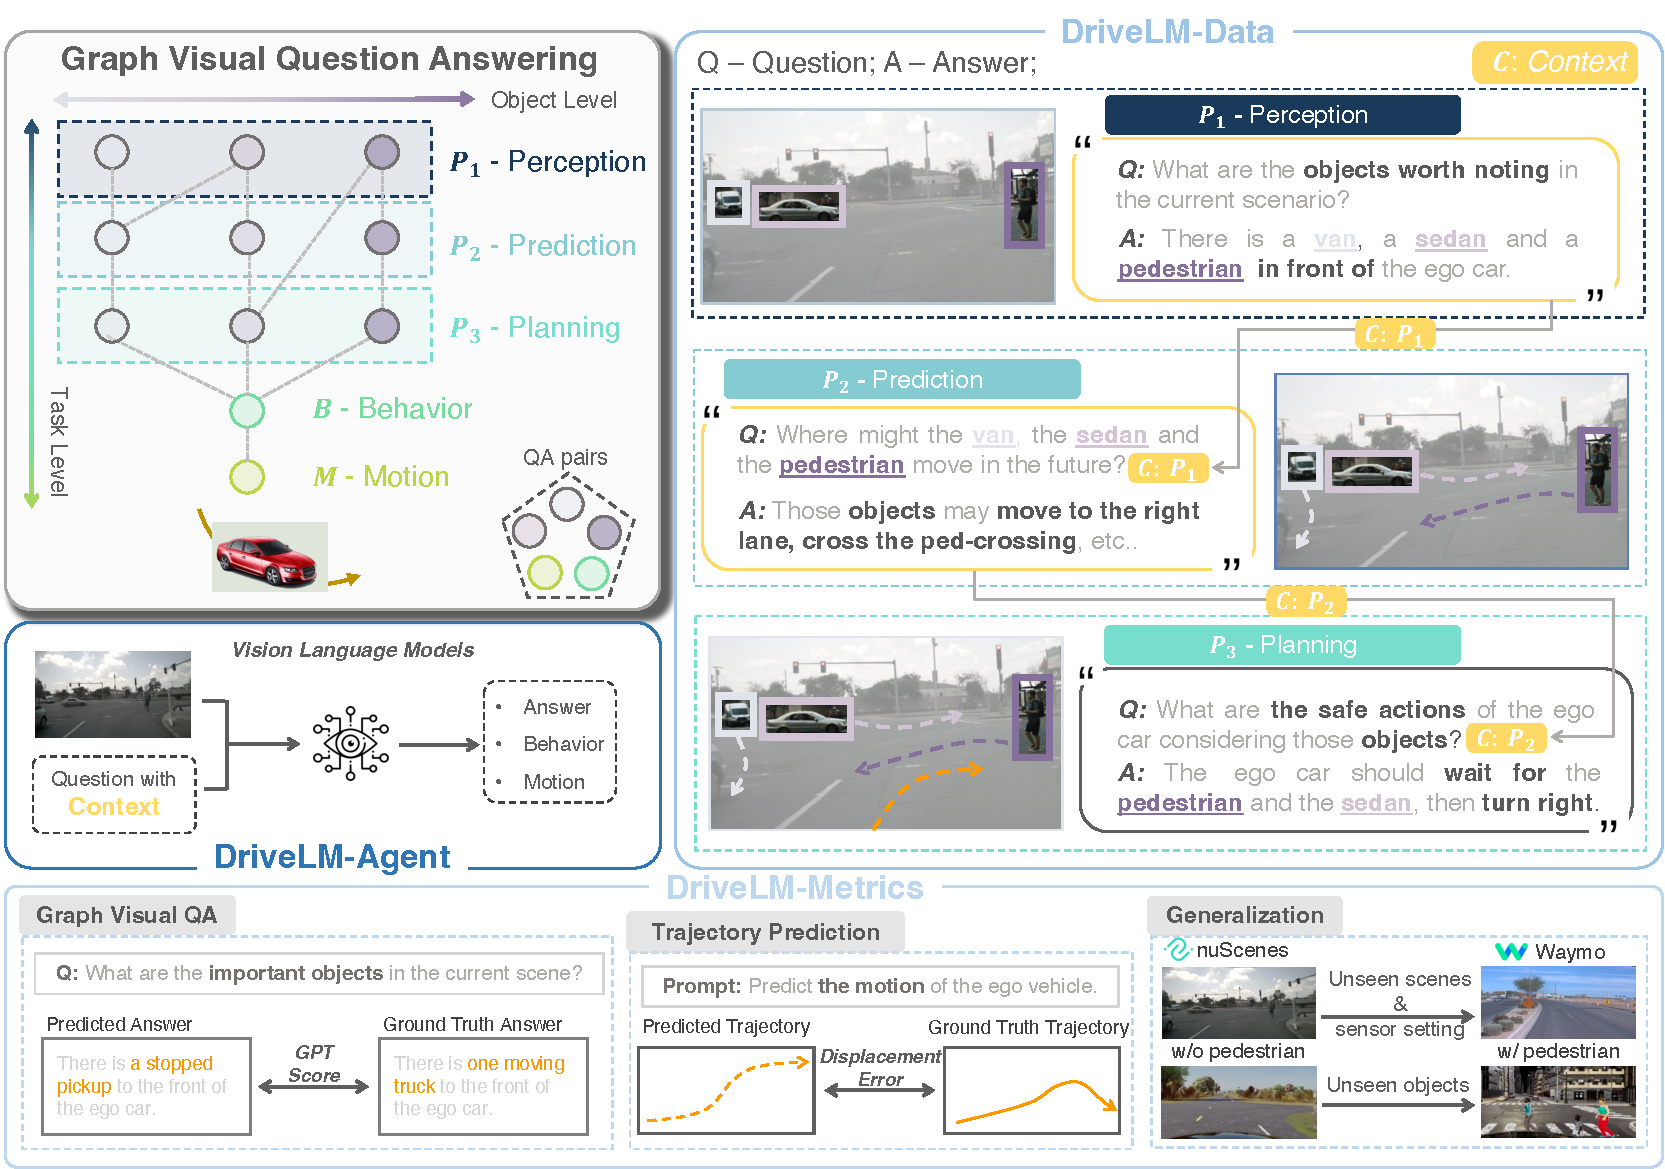
\includegraphics[width=\textwidth]{ch-drivelm/images/teaser_smch_v10.pdf}
  \caption[Overview of DriveLM: task, data, metrics and baseline]{\textbf{Overview of DriveLM}, a task, dataset, metrics and baseline for end-to-end autonomous driving. Inspired by~\cite{chen2024e2esurvey}, DriveLM considers Graph Visual Question Answering (GVQA), where QA pairs are interconnected via logical dependencies at the object level, \ie, interactions between object pairs, and at the task level, \eg, perception $\rightarrow$ prediction $\rightarrow$ planning $\rightarrow$ behaviour (a discretised action described in natural language) $\rightarrow$ motion (a continuous trajectory). DriveLM-Data is used to train DriveLM-Agent, a baseline for GVQA, whose effectiveness is validated with DriveLM-Metrics in challenging settings that require zero-shot generalisation.}
  \label{drivelm:fig:teaser}
\end{figure}

\section{Related Work}\label{drivelm:sec:related}

\paragraph{Generalisation in autonomous driving.}
The inadequate generalisation of driving systems to the ``long tail'' of corner cases poses significant safety concerns~\cite{chen2024e2esurvey,teng2023motion,tampuu2020survey}. Prior research tackles this issue primarily with data-driven methods~\cite{suo2021trafficsim,chen2022learning,akhauri2020enhanced,wang2021advsim,hanselmann2022king}; for example, TrafficSim~\cite{suo2021trafficsim} collects more data for safety-critical cases through simulation. An emerging direction leverages semantic information to supervise the detection of unseen or anomalous objects~\cite{elhafsi2023semantic,wang2023driveanywhere,chen2023categorical,pan2024vlp}. Even so, the zero-shot performance of driving systems is not yet satisfactory. This chapter explores a different route towards generalisation: learning logical reasoning through Graph VQA.

\paragraph{Language-grounded driving.}
Several concurrent methods feed multi-modal inputs into large language models (LLMs) for driving tasks~\cite{seff2023motionlm,mao2023gptdriver,chen2024drivingwithllms,jin2023adapt,xu2024drivegpt4,wayve2023lingo1,wang2023driveanywhere,marcu2023lingoqa,chen2023categorical,wang2023drivemlm,mao2023language,tian2024drivevlm,shao2024lmdrive,yuan2024ragdriver,pan2024vlp,han2024dmedriver}. GPT-Driver~\cite{mao2023gptdriver} and LLM-Driver~\cite{chen2024drivingwithllms} encode the perceived scene state into prompts and rely on LLMs to formulate reasonable plans. DriveGPT4~\cite{xu2024drivegpt4} projects raw sensor data into tokens and uses an LLM to predict control signals and explanations end to end. Despite these preliminary attempts, the potential of LLMs for generalisation in driving remains untapped. DriveLM combines VLMs with training on graph-structured QAs, which allows us to show benefits in zero-shot end-to-end planning, something these concurrent studies did not demonstrate.

\paragraph{Vision-language benchmarks for driving.}
Many driving datasets with language annotations have been proposed~\cite{zhou2023vision,Dewangan2023talk2bev,wu2023referkitti,wu2025nuprompt,qian2024nuscenesqa,kim2019had,kim2018bddx,sachdeva2023rank2tell,malla2023drama,marcu2023lingoqa,ding2024holistic}. Some of them express perceptual information as text: NuScenes-QA~\cite{qian2024nuscenesqa} and NuPrompt~\cite{wu2025nuprompt} describe the positions and states of surrounding objects. BDD-X~\cite{kim2018bddx} gives reasons for the actions of the ego vehicle in natural language, while DRAMA~\cite{malla2023drama} and Rank2Tell~\cite{sachdeva2023rank2tell} identify crucial objects and provide corresponding driving suggestions. These datasets, however, focus on scene-level context or on individual objects. DriveLM fills this gap by organising language annotations at the object level and the task level in a graph structure (Table~\ref{drivelm:tab:dataset}).

\paragraph{Embodied planning with LLMs.}
Recent work leverages the reasoning and generalisation capacity of LLMs~\cite{touvron2023llama,floridi2020gpt,kojima2022large} for embodied AI systems~\cite{brohan2023can,huang2022inner,zitkovich2023rt2,driess2023palme,liang2023code,karamcheti2023voltron,rana2023sayplan}. PaLM-E~\cite{driess2023palme} trains an LLM for various embodied tasks, including sequential robotic manipulation planning. Code as Policies~\cite{liang2023code} provides a robot-centric formulation of programs generated by language models and executed on real systems. RT-2~\cite{zitkovich2023rt2} represents robot actions as language tokens and trains VLMs to output robot policies. These methods show the capabilities of LLMs in embodied planning and inspire us to apply them to the shortcomings of generalisation in driving, which are far less explored.

\paragraph{Reasoning over graph structures.}
Reasoning is one of the basic forms of simulated human thinking: it derives new judgements from one or several existing ones~\cite{chen2020review}. Many reasoning methods are built on graphs~\cite{shi2019scenegraph,besta2023got,wang2019knowledgegraph,chen2019graph}. XNMs~\cite{shi2019scenegraph} use scene graphs for explainable and explicit reasoning with structured knowledge. KPRN~\cite{wang2019knowledgegraph} reasons over a knowledge graph for recommender systems. Graph of Thoughts~\cite{besta2023got} models the information generated by an LLM as an arbitrary graph, bringing LLM reasoning closer to brain mechanisms. Inspired by these works, DriveLM links the perception, prediction and planning stages of driving through a graph, so that a model can grasp the reasoning process and reason about unseen scenarios using the learned graph structure.

\section{Graph Visual Question Answering}\label{drivelm:sec:gvqa}

Human drivers usually decompose their decision-making into distinct stages that follow a logical progression: identifying and localising the key objects, anticipating their possible future actions and interactions, and planning the ego motion based on all of this information~\cite{macadam2003understanding,groeger2013understanding}. GVQA casts this progression as a proxy task that mimics the human reasoning process. This section formulates the task (Section~\ref{drivelm:sec:task}) and the metrics used to evaluate it (Section~\ref{drivelm:sec:metrics}); the datasets that instantiate it are described in Section~\ref{drivelm:sec:data}.

\subsection{Task Formulation}\label{drivelm:sec:task}

We organise all question-answer pairs (QAs) of an image frame into a graph. By ``graph-structured'' we mean a directed acyclic graph (DAG): a question can take context from several parent and grandparent nodes. The graph $G=(V,E)$ contains a set of vertices $V$, where each vertex is a QA pair $v=(q,a)$ associated with one or more key objects in the scene. What distinguishes GVQA from ordinary VQA is that its QAs have logical dependencies, which form the edges of the graph: $E\subseteq V\times V$ is a set of directed edges, and each edge $e=(v_p,v_c)$ connects a parent QA $v_p$ to a child QA $v_c$. The edge set is built along two dimensions. Object-level edges represent the impact of interactions between different objects; for example, in Fig.~\ref{drivelm:fig:teaser} (centre) the planning node for the sedan is influenced by the perception node of the pedestrian. Task-level edges capture the logical chain of reasoning stages:
\begin{itemize}
  \item \textbf{Perception} ($P_1$): identification, description and localisation of the key objects in the current scene.
  \item \textbf{Prediction} ($P_2$): estimation of the possible actions and interactions of the key objects, based on the perception results.
  \item \textbf{Planning} ($P_3$): possible safe actions of the ego vehicle.
  \item \textbf{Behaviour} ($B$): classification of the driving decision.
  \item \textbf{Motion} ($M$): waypoints of the future trajectory of the ego vehicle.
\end{itemize}

The concepts of perception, prediction and planning ($P_{1-3}$) are similar to those of end-to-end autonomous driving~\cite{chen2024e2esurvey}, while motion and behaviour are defined from the future trajectory of the ego vehicle. The motion $M$ is a sequence of $N$ future BEV positions. Point $i$ has coordinates $(x_i,y_i)$ relative to the current position: $M=\{(x_i,y_i)\}_{i=0}^{N}$. The displacement representation is
\begin{equation}
  \{x,y\}_{\text{dist}} = \{(\delta_{x,1},\delta_{y,1}),\ldots,(\delta_{x,N},\delta_{y,N})\},
  \label{drivelm:eq:xy_dist}
\end{equation}
where $\delta_{x,i}=x_i-x_{i-1}$ and $\delta_{y,i}=y_i-y_{i-1}$ for $i=1,2,\ldots,N$. The behaviour representation serves as an interface from $P_{1-3}$ to $M$. To obtain it, we map the mean of $x_{\text{dist}}$ and $y_{\text{dist}}$ to one of the predefined bins, where each bin corresponds to a category of either speed or steering, denoted $B_{sp}$ and $B_{st}$ respectively. We use five bins for each:
\begin{align*}
  B_{sp} &\in \{\texttt{fast}_2, \texttt{fast}_1, \texttt{moderate}, \texttt{slow}_1, \texttt{slow}_2\},\\
  B_{st} &\in \{\texttt{left}_2, \texttt{left}_1, \texttt{straight}, \texttt{right}_1, \texttt{right}_2\},
\end{align*}
where the subscript indicates the intensity. The speed and steering categories of a trajectory together form its behaviour category $B=(B_{sp},B_{st})$. This simple definition of $B$ is a starting point for research on driving with VLMs; the formulation also supports more abstract behaviours such as lane changes or overtaking.

\subsection{Evaluation Metrics}\label{drivelm:sec:metrics}

DriveLM-Metrics evaluate the three components of GVQA: motion $M$, behaviour $B$ and $P_{1-3}$. For motion, we use the standard metrics of the nuScenes and Waymo benchmarks, the average and final displacement errors (\textbf{ADE} and \textbf{FDE}) and the \textbf{collision rate} of the predicted trajectory, following UniAD~\cite{hu2023uniad}. For behaviour, we report the \textbf{classification accuracy}, with separate speed and steering accuracies.

For $P_{1-3}$, we use two metrics. \textbf{SPICE}~\cite{anderson2016spice} parses each answer into a semantic scene graph of objects, attributes and relations and computes tuple overlap; it remains limited by parsing errors and reference coverage. The \textbf{GPT Score} complements it with a model-based judgement: the question, ground-truth answer, predicted answer and a scoring prompt are sent to ChatGPT-3.5~\cite{ouyang2022training,chatgpt}, and a numerical score is parsed from the response. The GPT Score is an evaluation instrument rather than ground truth, and later audits found it sensitive to prompt context (Section~\ref{drivelm:sec:community}). Appendix~\ref{drivelm:app:metrics} defines the metrics and introduces conventional language metrics and a Completeness score.

\section{DriveLM-Data}\label{drivelm:sec:data}

To provide comprehensive and accurate QAs with the graph structure of Section~\ref{drivelm:sec:task}, we build two datasets, DriveLM-nuScenes and DriveLM-CARLA. Because nuScenes and CARLA differ substantially, the two datasets are collected with different pipelines (Fig.~\ref{drivelm:fig:data_collection}) and have different statistics (Table~\ref{drivelm:tab:dataset}). An official evaluation server with a public leaderboard benchmarks methods on the task (Section~\ref{drivelm:sec:community}).

\begin{figure}[t]
  \centering
  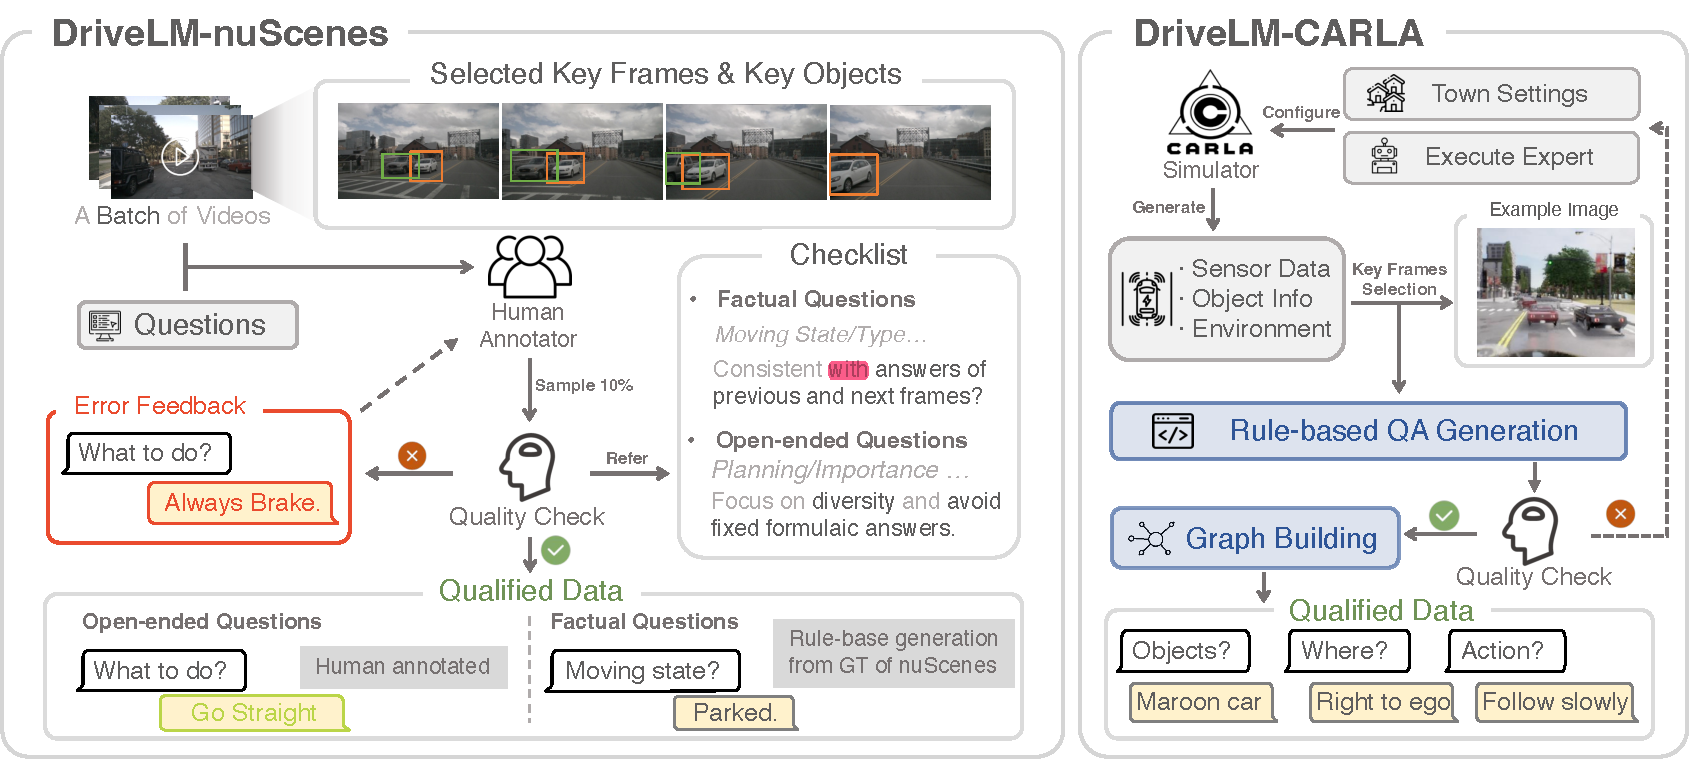
\includegraphics[width=\linewidth]{ch-drivelm/images/data_v8_1_smch_revised.pdf}
  \caption[Annotation pipelines of DriveLM-nuScenes and DriveLM-CARLA]{\textbf{Annotation pipelines.} DriveLM-nuScenes adopts a semi-rule-based QA labelling pipeline that uses both the ground-truth annotations of nuScenes and OpenLane-V2 and feedback from human annotators. A critical part of the pipeline is the multi-round quality check, which guarantees high data quality at reasonable cost. DriveLM-CARLA meets the same standards with a fully rule-based QA labelling pipeline, using the rule-based expert PDM-Lite~\cite{beisswenger2024pdmlite}.}
  \label{drivelm:fig:data_collection}
\end{figure}

\begin{table}[t]
  \centering
  \caption[Comparison of DriveLM-Data with existing driving-language datasets]{\textbf{Comparison of DriveLM-nuScenes and DriveLM-CARLA with existing datasets.} DriveLM-Data significantly advances annotation quantity, comprehensiveness (covering \textbf{perception, prediction and planning}) and logic (from chain to \textbf{graph}). \dag: full dataset; \ddag: keyframe dataset; $^{*}$: semi-rule-based labelling (with human annotators); $^{**}$: fully rule-based labelling (no human annotators); -: publicly unavailable.}
  \label{drivelm:tab:dataset}
  \small
  \begin{adjustbox}{max width=\textwidth}
  \begin{tabular}{l|ccc|ccc|c}
    \toprule
    \textbf{Dataset} & \makecell{\textbf{Source}\\\textbf{Dataset}} & \textbf{\# Frames} & \makecell{\textbf{Avg. QA}\\\textbf{per Frame}} & \textbf{Perception} & \textbf{Prediction} & \textbf{Planning} & \textbf{Logic} \\
    \midrule
    nuScenes-QA~\cite{qian2024nuscenesqa} & nuScenes & 34,149 & 13.5 & 460k$^{**}$ & \ding{55} & \ding{55} & None \\
    nuPrompt~\cite{wu2025nuprompt} & nuScenes & 34,149 & 1.0 & 35k$^{*}$ & \ding{55} & \ding{55} & None \\
    HAD~\cite{kim2019had} & HDD & 25,549 & 1.8 & 25k & \ding{55} & 20k & None \\
    BDD-X~\cite{kim2018bddx} & BDD & 26,228 & 1 & 26k & \ding{55} & \ding{55} & None \\
    LingoQA~\cite{marcu2023lingoqa} & LingoQA & 28,000 & 15.3 & - & - & - & None \\
    DRAMA~\cite{malla2023drama} & DRAMA & 17,785 & 5.8 & 85k & \ding{55} & 17k & Chain \\
    Rank2Tell~\cite{sachdeva2023rank2tell} & Rank2Tell & 5,800 & - & - & \ding{55} & - & Chain \\
    \midrule
    \rowcolor[gray]{0.95} DriveLM-nuScenes & nuScenes & 4,871 & \textbf{91.4} & 144k$^{*}$ & 153k & 146k & \textbf{Graph} \\
    \rowcolor[gray]{0.95} DriveLM-CARLA\dag & CARLA & 64,285 & 24.4 & 697k$^{**}$ & 311k$^{**}$ & 558k$^{**}$ & \textbf{Graph} \\
    \rowcolor[gray]{0.95} DriveLM-CARLA\ddag & CARLA & 5,721 & 24.8 & 63k$^{**}$ & 28k$^{**}$ & 51k$^{**}$ & \textbf{Graph} \\
    \bottomrule
  \end{tabular}
  \end{adjustbox}
\end{table}

\subsection{DriveLM-nuScenes}\label{drivelm:sec:data_nus}

We divide the annotation process into three steps: selecting key frames from video clips, choosing key objects within these key frames, and annotating the frame-level $P_{1-3}$ QAs for the key objects. Part of the perception QAs are generated from the ground truth of nuScenes~\cite{caesar2020nuscenes} and OpenLane-V2~\cite{wang2023openlanev2}; the remaining QAs are annotated manually. The question templates for manual annotation were designed by five domain experts to reflect how humans make driving decisions. Annotators are shown all question templates for each frame and encouraged to answer all of them, with a skip option for questions that do not apply.

Because most of DriveLM-nuScenes is annotated manually, quality control is particularly important. In each review round, the data are divided into batches and ten percent of each batch is inspected; a batch that falls below the qualification threshold is returned for relabelling. The threshold and inter-annotator agreement were not reported, so this procedure documents the workflow rather than establishing a measured label-error rate. The resulting dataset has 4,072 training frames and 799 validation frames. It contains more text annotations per frame and a more complex graph structure than the datasets listed in Table~\ref{drivelm:tab:dataset}; its QAs cover perception, prediction and planning. Appendix~\ref{drivelm:app:nuscenes} details its composition, annotation protocol and statistics.

\subsection{PDM-Lite: An Expert Driver for CARLA Leaderboard 2.0}\label{drivelm:sec:data_expert}

We collect DriveLM-CARLA with CARLA 0.9.14 in the Leaderboard 2.0 framework~\cite{dosovitskiy2017carla}. Leaderboard 2.0 contains a large set of new driving scenarios compared with its predecessor, Leaderboard 1.0, but at the time of this work no method existed to collect training data at scale in it. For example, the privileged rule-based expert used by TransFuser++~\cite{jaeger2023hidden}, a state-of-the-art method on Leaderboard 1.0, obtains a Driving Score (DS) of only 2\% on the 8+ kilometre-long official validation routes of Leaderboard 2.0. DriveLM-CARLA is therefore collected with PDM-Lite, a rule-based expert for CARLA Leaderboard 2.0 developed for this purpose by Bei{\ss}wenger~\cite{beisswenger2024pdmlite}. At the time of publication, it was the first working rule-based expert for Leaderboard 2.0, and it handles the new challenges of this leaderboard. It is similar to PDM-Closed~\cite{dauner2023parting}, a rule-based planner for nuPlan~\cite{caesar2021nuplan}. PDM-Lite uses the Intelligent Driver Model (IDM)~\cite{treiber2000idm} to obtain a target speed based on the leading vehicle, pedestrian, stop sign or traffic light. Unlike PDM-Closed, which selects one of 16 proposals with a complex cost function, PDM-Lite uses only two proposals and a simpler cost function based on the TransFuser++ expert~\cite{jaeger2023hidden}. The result is a lightweight planner suitable for scalable QA generation. On the 20 official validation routes, Table~\ref{drivelm:tab:pdm_results} preserves a route-pooled average DS of 36.3 and a pooled route--seed dispersion of 28.1. The original paper's main text separately quotes 44\% without identifying a matching protocol. The three seed-level aggregate scores and exact evaluation configuration are unavailable, so 36.3 and 44\% remain distinct source reports rather than a single resolved estimate.

\subsection{DriveLM-CARLA}\label{drivelm:sec:data_carla}

To collect DriveLM-CARLA, we set up routes in urban, residential and rural areas and execute PDM-Lite on them. During this process, we record the necessary sensor data, sample keyframes, generate QAs from privileged information about the objects and the scene, and connect the QAs into a graph according to their logical relationships. Data and labels are generated at 4 FPS, and keyframes are extracted when the decision of the expert changes, \eg, from accelerating to braking. The rule-based annotation pipeline is illustrated in Fig.~\ref{drivelm:fig:data_collection}. During collection, we extract privileged information from the simulator about the state of static and dynamic objects in the scene and about the rules triggered in the expert. We use all 38 scenarios of Leaderboard 2.0 except \mbox{\emph{InterurbanAdvancedActorFlow}}, \mbox{\emph{MergerIntoSlowTraffic}} and \mbox{\emph{VehicleTurningRoute}}, and create questions and answers from the extracted information with hand-crafted sentence templates. The questions and their graph structure are given in Appendix~\ref{drivelm:app:carla}. This annotation process scales easily, since only the route and scenario settings need to be defined in CARLA and all subsequent steps run automatically. With 1.6M QAs obtained through this straightforward scaling recipe, DriveLM-CARLA is the largest driving-language benchmark in Table~\ref{drivelm:tab:dataset} in terms of total textual content.

\section{DriveLM-Agent: A GVQA Baseline}\label{drivelm:sec:agent}

DriveLM-Agent is a baseline for GVQA built on a general VLM, so that it can exploit the knowledge acquired during pre-training. Its goal is to translate an image into the desired motion of the ego vehicle ($M$) through the VQA stages $P_1$, $P_2$, $P_3$ and $B$. We choose BLIP-2~\cite{li2023blip2} as the base VLM because of its simple architecture and flexible fine-tuning, but the approach can be applied to other VLMs as well.

As shown in Fig.~\ref{drivelm:fig:model_pipeline}, DriveLM-Agent works in stages. (1) The $P_{1-3}$ stages, \ie, perception, prediction and planning, form the foundation: they interpret the scene and reason about its structure. (2) The behaviour stage aggregates the crucial information from $P_{1-3}$ into a description of the desired driving action in language. (3) The motion stage translates this behaviour into an executable driving trajectory. The logical dependency between linked QAs is implemented through context passed between connected nodes of the graph, as described next.

\begin{figure}[t]
  \centering
  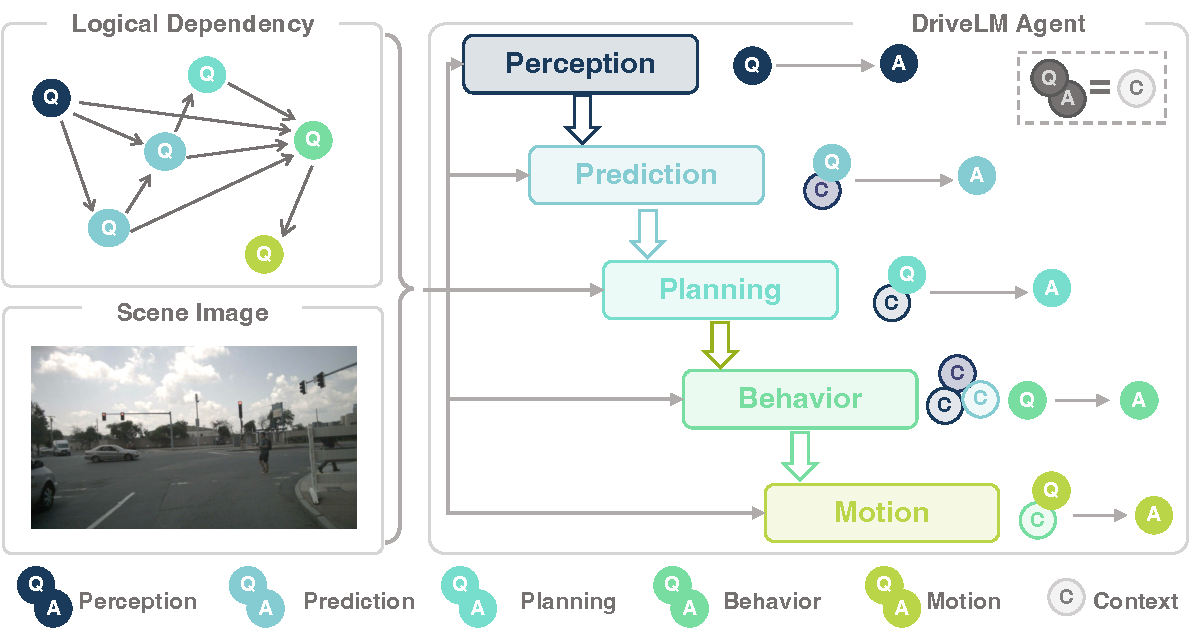
\includegraphics[width=0.8\linewidth]{ch-drivelm/images/model_pipeline_smch_v1.pdf}
  \caption[Pipeline of DriveLM-Agent]{\textbf{Pipeline of DriveLM-Agent.} Given the scene image, a VLM performs prompting with context to model the logical dependency among the five QA stages. Context is built from preceding QAs and can have one or more sources.}
  \label{drivelm:fig:model_pipeline}
\end{figure}

\subsection{Prompting with Context}\label{drivelm:sec:context}

Directly translating images into motion, as in~\cite{Prakash2021transfuser,chitta2021neat}, is extremely challenging. Motivated by the multi-step reasoning of humans, we adopt a similar strategy for VLM-based driving, which facilitates the retrieval of knowledge stored in LLMs and improves explainability. The model uses the answers of earlier steps of the reasoning process as \emph{context} for later questions. For each edge $e=(v_p,v_c)\in E$, we append the QA of the parent node $v_p$ to the question of the current node $v_c$, with the prefix ``\emph{Context:}''. If a node has several parents, their QAs are concatenated into one context sequence. Context is only one possible way to implement the logical dependencies of GVQA; we choose it for its simplicity. With this scheme, relevant information is passed forward along the logical dependencies established by the graph. During training, the ground-truth parent QAs serve as context (teacher forcing); at inference, the model is applied in multiple rounds in the order $P_1$, $P_2$, $P_3$, $B$, $M$, so that each stage receives the predicted answers of the preceding stages (Appendix~\ref{drivelm:app:agent}).

The size and structure of the graph at inference time are a design choice that can be adapted to the task or to the available compute budget. We use this property to train on all available QAs but to perform inference on specific subgraphs whose questions are sampled with heuristics (Appendix~\ref{drivelm:app:impl}).

\paragraph{Context aggregation through behaviour.}
Driving encompasses a wide array of situations that require an appropriate response. Despite this diversity, almost all of them involve decisions that can be discretised into a set of behaviours. For example, braking appropriately addresses situations as different as a red light, a stop sign or an object ahead of the vehicle. The behaviour stage generates such a behaviour: a statement in natural language that articulates the intended movement of the vehicle. As described in Section~\ref{drivelm:sec:task}, this description serves as a reflective step in which the model summarises all crucial information from the graph. We therefore use all possible sources of context for predicting the behaviour, \ie, all QAs in $P_{1-3}$. We observe empirically that this design is crucial for driving with VLMs.

\subsection{Trajectory Tokenisation for Motion}\label{drivelm:sec:traj_token}

General VLMs cannot easily output fine-grained numerical values. RT-2~\cite{zitkovich2023rt2} handles robotic actions with a specialised trajectory tokenisation module, and we adopt this approach so that DriveLM-Agent can take the image and the behaviour description as input and output a trajectory. Specifically, we divide the waypoint coordinates into 256 bins, determined empirically from the statistics of the training trajectories. We re-define tokens of the BLIP-2 language tokeniser so that each bin has its own token, and fine-tune the VLM on the re-defined vocabulary (Appendix~\ref{drivelm:app:agent}). For simplicity, the motion stage uses the same VLM architecture (BLIP-2), but with independent LoRA weights, trained on a dataset that contains only the QAs of the motion stage. This functionality could therefore equally be provided by a lightweight LLM~\cite{radford2019language} or by a driving-specific architecture that accepts a command as input~\cite{hu2022stp3,wu2022tcp}.

\section{Experiments}\label{drivelm:sec:experiments}

The experiments address five questions. (1) How can VLMs be effectively repurposed for end-to-end autonomous driving? (2) Can VLMs for driving generalise when evaluated with unseen sensor setups? (3) Can they generalise to an object class never seen during training? (4) What is the effect of each question in perception, prediction and planning on the final behaviour decision? (5) How well do VLMs perform perception, prediction and planning via GVQA? Further results, including other base VLMs, are given in Appendix~\ref{drivelm:app:exp}.

\paragraph{Setup.}
All fine-tuning uses LoRA~\cite{hu2021lora}. For DriveLM-nuScenes, BLIP-2 is fine-tuned on the \texttt{train} split for 10 epochs with a batch size of 2 per GPU, taking approximately 7 hours on 8 V100 GPUs. For DriveLM-CARLA, BLIP-2 is trained on the \texttt{train} keyframes for 6 epochs, taking 6 hours on 4 A100 GPUs. Appendix~\ref{drivelm:app:impl} gives further details.

\subsection{VLMs for End-to-End Driving}\label{drivelm:sec:exp_arch}

The first experiment assesses the ability of VLMs to perform open-loop planning on DriveLM-nuScenes, and in particular the impact of the context provided to the behaviour and motion stages. Given the sensor data (and, for VLM methods, a text input), the model predicts the future trajectory of the ego vehicle as waypoints. Open-loop planning suffers from a mismatched data distribution~\cite{li2024ego}; we alleviate this by evaluating only on the key frames annotated in DriveLM-nuScenes.

\paragraph{Baselines.}
As a reference for the difficulty of the task, we provide a simple \textbf{Command Mean} baseline. Each frame in nuScenes is associated with one of three commands, `turn left', `turn right' or `go straight', and the baseline outputs the mean of all training trajectories whose command matches that of the test frame. We also compare with UniAD~\cite{hu2023uniad}, the state of the art on nuScenes. Besides its original setting, which requires video input, we train a single-frame version (\textbf{UniAD-Single}) for a fair comparison. Finally, \textbf{BLIP-RT-2} denotes BLIP-2~\cite{li2023blip2} fine-tuned on DriveLM-Data with the trajectory tokenisation of Section~\ref{drivelm:sec:traj_token} for the motion task only. It indicates the performance of the same network architecture as DriveLM-Agent without context inputs or VQA training data.

\paragraph{DriveLM-Agent variants.}
We consider three variants that add the proposed components step by step: (1) a two-stage version that predicts the behaviour and then the motion (Section~\ref{drivelm:sec:task}) but uses no $P_{1-3}$ context for behaviour prediction (`None'); (2) a `Chain' version that builds the $P_{1-3}$ graph but passes only its final node ($P_3$) to the behaviour stage; and (3) the full model (`Graph'), which uses all QAs of $P_{1-3}$ as context for $B$.

\begin{table}[t]
  \centering
  \caption[Open-loop planning on nuScenes and transfer to Waymo]{\textbf{Open-loop planning on DriveLM-nuScenes and zero-shot transfer to Waymo.} The Waymo column marked $U^{\dagger}$ preserves a source-reported quantity whose identity is unresolved; it is not used here as either collision rate or FDE. All rows are single runs.}
  \label{drivelm:tab:arch}
  \setlength{\tabcolsep}{3pt}
  \begin{adjustbox}{max width=\textwidth}
  \begin{tabular}{l|cc|ccc|cc|ccc|cc}
    \toprule
    \multirow{3}{*}{\textbf{Method}} & \textbf{Behaviour} & \textbf{Motion} & \multicolumn{5}{c|}{\textbf{nuScenes}} & \multicolumn{5}{c}{\textbf{Waymo}} \\
    \cmidrule(lr){4-8}\cmidrule(lr){9-13}
    & \textbf{($B$)} & \textbf{($M$)} & \multicolumn{3}{c|}{\textbf{Behaviour ($B$)}} & \multicolumn{2}{c|}{\textbf{Motion ($M$)}} & \multicolumn{3}{c|}{\textbf{Behaviour ($B$)}} & \multicolumn{2}{c}{\textbf{Motion ($M$)}} \\
    & \textbf{Context} & \textbf{Context} & Acc.\,$\uparrow$ & Speed\,$\uparrow$ & Steer\,$\uparrow$ & ADE\,$\downarrow$ & Col.\,$\downarrow$ & Acc.\,$\uparrow$ & Speed\,$\uparrow$ & Steer\,$\uparrow$ & ADE\,$\downarrow$ & $U^{\dagger}$\,$\downarrow$ \\
    \midrule
    Command Mean & - & - & - & - & - & 4.57 & 5.72 & - & - & - & 7.98 & 11.41 \\
    UniAD-Single & - & - & - & - & - & 1.80 & 2.62 & - & - & - & 4.16 & 9.31 \\
    BLIP-RT-2 & - & - & - & - & - & 2.63 & 2.77 & - & - & - & 2.78 & 6.47 \\
    \midrule
    \rowcolor[gray]{0.9} & None & $B$ & \textbf{61.45} & \textbf{72.20} & \textbf{84.73} & \textbf{1.39} & \textbf{1.67} & 35.70 & 43.90 & 65.20 & 2.76 & 6.59 \\
    \rowcolor[gray]{0.9} DriveLM-Agent & Chain & $B$ & 50.43 & 60.32 & 75.34 & 2.07 & 2.08 & 34.62 & 41.28 & 64.55 & 2.85 & 6.89 \\
    \rowcolor[gray]{0.9} & Graph & $B$ & 57.49 & 69.89 & 80.63 & 1.74 & 1.89 & \textbf{39.73} & \textbf{54.29} & \textbf{70.35} & \textbf{2.63} & \textbf{6.17} \\
    \midrule
    \textit{UniAD}~\cite{hu2023uniad} & \textit{-} & \textit{-} & \textit{-} & \textit{-} & \textit{-} & \textit{0.80} & \textit{0.17} & \textit{-} & \textit{-} & \textit{-} & \textit{-} & \textit{-} \\
    \bottomrule
  \end{tabular}
  \end{adjustbox}
  \par\smallskip
  {\linespread{1.1}\footnotesize\raggedright
  This column preserves a source quantity labelled `Col.' here and `FDE' in Table~\ref{drivelm:tab:waymo_supp}. The evaluator outputs and units are unavailable, so it is denoted $U$ and excluded from motion claims.\par}
\end{table}

\paragraph{Results.}
Table~\ref{drivelm:tab:arch} shows the results. Among the baselines, BLIP-RT-2 does not match UniAD-Single on nuScenes, although both outperform Command Mean. Introducing behaviour as an intermediate representation improves the single-run open-loop results over BLIP-RT-2. Graph context, however, does not improve on the no-context DriveLM-Agent in this in-domain setting: ADE changes from 1.39 to 1.74 and the reported collision rate from 1.67 to 1.89. The original video-based UniAD remains better, but it uses privileged temporal input.

\subsection{Generalisation Across Sensor Configurations}\label{drivelm:sec:exp_waymo}

As a more challenging setting, we apply the models of Section~\ref{drivelm:sec:exp_arch} without further training to a new domain, the Waymo Open Dataset~\cite{sun2020waymo}. Waymo does not include images from rear cameras, so we drop this input for UniAD-Single. The VLM methods use only the front view and do not require any adaptation. Since Waymo has no GVQA annotations, the questions are generated with rules (Appendix~\ref{drivelm:app:impl}).

\paragraph{Results.}
As shown in Table~\ref{drivelm:tab:arch}, the single-run Waymo ADE of UniAD-Single is worse than that of BLIP-RT-2. This comparison is confounded: UniAD-Single loses its rear-camera input because Waymo lacks those images, whereas the VLM uses only a front view by design; the models also differ greatly in scale and pre-training. Most of the observed gap therefore cannot be attributed to the graph. BLIP-RT-2, which has neither VQA training nor context, reaches an ADE of 2.78 against 4.16 for UniAD-Single, and DriveLM-Agent without context reaches 2.76. Full graph context reaches 2.63, while prediction-only context reaches 2.62 in Table~\ref{drivelm:tab:waymo_supp}; thus the full graph is not needed for the best displayed ADE. Its clearest displayed gain is speed accuracy, from 43.90 without context to 54.29 with full context. These values come from one training run and do not isolate graph structure from model and input differences. The unresolved $U$ column is not interpreted until its metric identity is recovered.

Fig.~\ref{drivelm:fig:qualitative} shows qualitative results of DriveLM-Agent on nuScenes and Waymo. The model generally gives intuitive answers, with a few exceptions (\eg, planning on DriveLM-nuScenes and perception on Waymo), which shows the utility of GVQA for interactive driving systems. On Waymo, the prediction and planning answers are meaningful despite the imperfect perception. More visualisations are given in the original paper~\cite{sima2024drivelm}.

\begin{figure}[t]
  \centering
  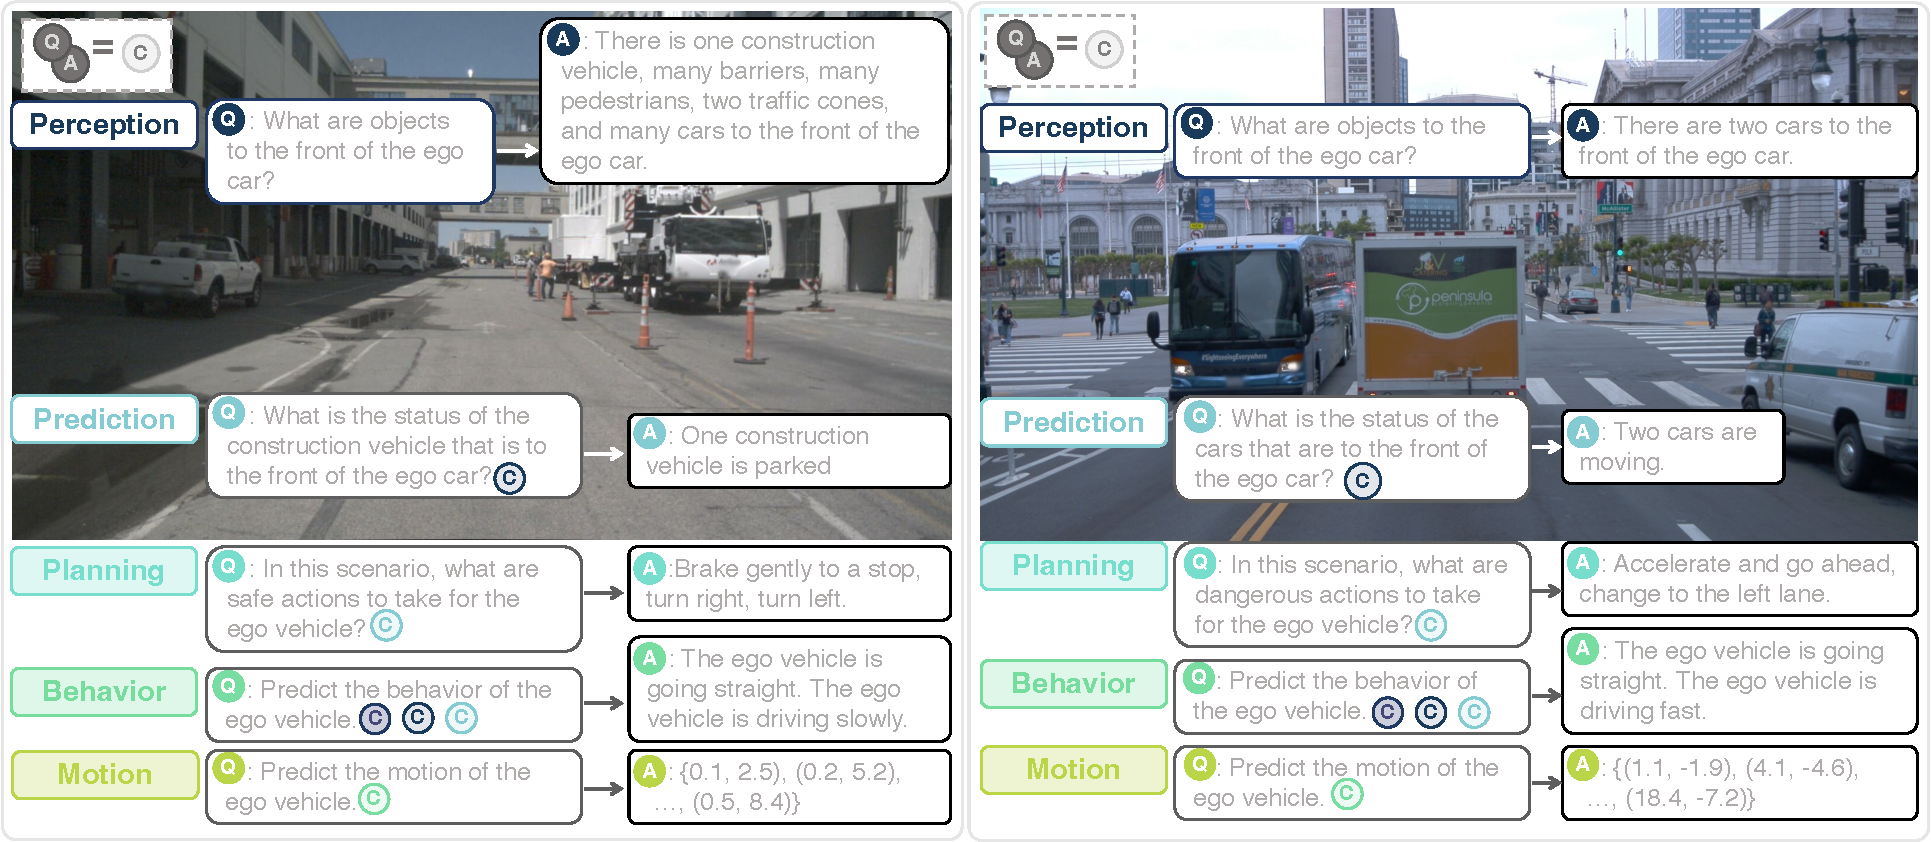
\includegraphics[width=\textwidth]{ch-drivelm/images/qualitative_smch_v7.pdf}
  \caption[Qualitative results of DriveLM-Agent on nuScenes and Waymo]{\textbf{Qualitative results of DriveLM-Agent.} Left: a DriveLM-nuScenes \texttt{val} frame. Right: a Waymo \texttt{val} frame. We show the questions (Q), context (C) and predicted answers (A). The outputs of DriveLM-Agent are easy for human users to interpret.}
  \label{drivelm:fig:qualitative}
\end{figure}

\subsection{Generalisation to Unseen Objects}\label{drivelm:sec:exp_carla}

Next, we evaluate zero-shot generalisation to a novel object class. DriveLM-CARLA is collected without any pedestrians in its training and validation splits. We therefore generate a new test set, DriveLM-CARLA-ped, which consists only of frames in which a pedestrian is present in the scene; the correct behaviour is to stop for the pedestrian.

\paragraph{Baselines.}
We compare DriveLM-Agent with TransFuser++~\cite{jaeger2023hidden}, the state of the art on CARLA. Compared with DriveLM-Agent, TransFuser++ uses a larger input image, an additional LiDAR sensor and several driving-specific annotations (depth, semantics, 3D bounding boxes and HD map). Because of these task-specific inputs and outputs, however, TransFuser++ can only be trained on the base DriveLM-CARLA dataset and cannot incorporate general computer vision data during training, which makes generalisation more challenging.

\paragraph{DriveLM-Agent variants.}
Taking advantage of the more general architecture of a VLM, we train DriveLM-Agent on samples from COCO~\cite{lin2014microsoft} and GQA~\cite{hudson2019gqa} together with DriveLM-CARLA. We compare several versions: (1) adding a pedestrian-specific $P_1$ question to the graph at inference time, whose answer determines a follow-up question on how the ego vehicle should act, with the answer to the latter appended to the context of the behaviour question (`+ Pedestrian QA'); and (2) as an upper bound, feeding the ground-truth $P_{1-3}$ graph to the model at inference time instead of its own predictions (`GT'). The exact questions are given in Appendix~\ref{drivelm:app:impl}.

\begin{table}[t]
  \centering
  \caption[Generalisation to unseen pedestrians in DriveLM-CARLA]{\textbf{Response to a pedestrian class absent from DriveLM-CARLA training.} The test set contains pedestrian-crossing frames whose correct speed response is to stop. A pedestrian-specific question raises the displayed speed/behaviour accuracy, but the question is written with knowledge of the missing class and no stop-always baseline is reported. Rows in italics use ground-truth context.}
  \label{drivelm:tab:carla}
  \begin{adjustbox}{max width=\textwidth}
  \begin{tabular}{l|ccc|ccc}
    \toprule
    \multirow{2}{*}{\textbf{Method}} & \multicolumn{3}{c|}{\textbf{DriveLM-CARLA} ($B$)} & \multicolumn{3}{c}{\textbf{DriveLM-CARLA-ped} ($B$)} \\
    \cmidrule(lr){2-4}\cmidrule(lr){5-7}
    & Acc.\,$\uparrow$ & Spd.\,$\uparrow$ & Str.\,$\uparrow$ & Acc.\,$\uparrow$ & Spd.\,$\uparrow$ & Str.\,$\uparrow$ \\
    \midrule
    TransFuser++~\cite{jaeger2023hidden} & \textbf{70.19} & \textbf{73.29} & \textbf{90.68} & 8.72 & 8.72 & 100.00 \\
    \midrule
    \rowcolor[gray]{0.9} DriveLM-Agent & 59.63 & 61.50 & 78.26 & 4.59 & 4.59 & 100.00 \\
    \rowcolor[gray]{0.9} \quad + Pedestrian QA & 52.17 & 55.28 & 77.64 & \textbf{27.04} & \textbf{27.04} & 100.00 \\
    \midrule
    \textit{DriveLM-Agent (GT)} & \textit{60.25} & \textit{65.22} & \textit{80.12} & \textit{20.92} & \textit{20.92} & \textit{100.00} \\
    \textit{\quad + Pedestrian QA} & \textit{60.25} & \textit{65.22} & \textit{80.12} & \textit{92.35} & \textit{92.35} & \textit{100.00} \\
    \bottomrule
  \end{tabular}
  \end{adjustbox}
\end{table}

\paragraph{Results.}
Table~\ref{drivelm:tab:carla} presents the results. On the pedestrian test set, TransFuser++ drops from 70.19 on DriveLM-CARLA to 8.72, while DriveLM-Agent drops from 59.63 to 4.59. Adding the pedestrian QA raises the displayed accuracy to 27.04 but lowers accuracy on regular scenes from 59.63 to 52.17. This is evidence of sensitivity to a targeted prompt, not a balanced test of open-ended unseen-object competence: the question is written for the missing class, the model is co-trained on COCO and GQA, and the test contains only crossing pedestrians for which stopping is always the correct speed response. A stop-always control is not reported. With privileged ground-truth context, the score on pedestrian frames changes from 20.92 to 92.35. All are single-run results; the steering score is always 100 because every scene is on a straight road.

\subsection{Question-wise Analysis on DriveLM-nuScenes}\label{drivelm:sec:exp_question_wise}

Next, we analyse the effect of each type of QA on behaviour prediction when it is added as context. We first select a set of representative QAs for each stage. We then train BLIP-2 on different combinations of these sets, which are added as context for the behaviour question (Table~\ref{drivelm:tab:question_wise}).

\paragraph{Representative questions.}
The representative questions of each stage are:
\begin{itemize}[leftmargin=4.4em, labelwidth=3.8em, labelsep=0.6em, align=left, itemsep=0pt]
  \item[$P_{1-1}$:] What are the important objects in the current scene?
  \item[$P_{1-2}$:] What is the moving status of object \emph{X}?
  \item[$P_{1-3}$:] What is the visual description of object \emph{X}?
  \item[$P_{2-1}$:] What is the future state of object \emph{X}?
  \item[$P_{2-2}$:] Would object \emph{X} be in the moving direction of the ego vehicle?
  \item[$P_{2-3}$:] What object should the ego vehicle notice first / second / third when the ego vehicle is getting to the next possible location?
  \item[$P_{3-1}$:] What actions could the ego vehicle take based on the observation of object \emph{X}?
  \item[$P_{3-2}$:] What actions taken by the ego vehicle can lead to a collision with object \emph{X}?
  \item[$P_{3-3}$:] In this scenario, what are safe actions to take for the ego vehicle?
\end{itemize}
We choose these questions for two reasons: statistically, they make up about 60\% of all QAs in the three stages; subjectively, they represent most of the information a human needs to drive. A coarser, stage-wise analysis is given in Appendix~\ref{drivelm:app:waymo_ablation}.

\begin{table}[t]
  \centering
  \caption[Question-wise analysis on DriveLM-nuScenes]{\textbf{Question-wise analysis on DriveLM-nuScenes.} The questions $P_{x-y}$ are listed in Section~\ref{drivelm:sec:exp_question_wise}. Using the QAs of the prediction and planning stages as context for the behaviour question improves the performance over using perception only, whereas different questions within the same stage differ only slightly.}
  \label{drivelm:tab:question_wise}
  \begin{adjustbox}{max width=\textwidth}
  \begin{tabular}{c|ccc|ccc|ccc|ccc}
    \toprule
    \multirow{2}{*}{\textbf{ID}} & \multicolumn{3}{c|}{\textbf{Perception}} & \multicolumn{3}{c|}{\textbf{Prediction}} & \multicolumn{3}{c|}{\textbf{Planning}} & \multicolumn{3}{c}{\textbf{Behaviour}} \\
    & $P_{1-1}$ & $P_{1-2}$ & $P_{1-3}$ & $P_{2-1}$ & $P_{2-2}$ & $P_{2-3}$ & $P_{3-1}$ & $P_{3-2}$ & $P_{3-3}$ & Acc.\,$\uparrow$ & Speed\,$\uparrow$ & Steer\,$\uparrow$ \\
    \midrule
    1 & \checkmark & - & - & - & - & - & - & - & - & 54.69 & 66.83 & 75.22 \\
    2 & \checkmark & \checkmark & - & - & - & - & - & - & - & 55.32 & 67.33 & 74.34 \\
    3 & \checkmark & \checkmark & \checkmark & - & - & - & - & - & - & 53.94 & 65.33 & 75.72 \\
    \midrule
    4 & \checkmark & \checkmark & \checkmark & \checkmark & - & - & - & - & - & 58.82 & 71.83 & \textbf{80.98} \\
    5 & \checkmark & \checkmark & \checkmark & \checkmark & \checkmark & - & - & - & - & 57.07 & 71.96 & 78.97 \\
    6 & \checkmark & \checkmark & \checkmark & \checkmark & \checkmark & \checkmark & - & - & - & 57.70 & 72.22 & 79.22 \\
    \midrule
    7 & \checkmark & \checkmark & \checkmark & \checkmark & \checkmark & \checkmark & \checkmark & - & - & \textbf{58.95} & 72.59 & 80.23 \\
    8 & \checkmark & \checkmark & \checkmark & \checkmark & \checkmark & \checkmark & \checkmark & \checkmark & - & 57.95 & \textbf{72.97} & 79.97 \\
    9 & \checkmark & \checkmark & \checkmark & \checkmark & \checkmark & \checkmark & \checkmark & \checkmark & \checkmark & 57.49 & 69.89 & 80.63 \\
    \bottomrule
  \end{tabular}
  \end{adjustbox}
\end{table}

\paragraph{Results.}
Table~\ref{drivelm:tab:question_wise} shows the results. Training with QAs from the prediction and planning stages (IDs 4--9) improves the performance over training with perception QAs only (IDs 1--3). Adding QAs from the planning stage (IDs 7--9) does not significantly boost the performance compared with the preceding stage (IDs 4--6). A possible reason is that the future states of other vehicles already contain all the information needed for the behaviour decision.

\subsection{Performance for \texorpdfstring{$P_{1-3}$}{P1-3} via GVQA}\label{drivelm:sec:exp_vqa}

Finally, we establish baseline results for the $P_{1-3}$ stages of GVQA and study the impact of context. We use two VLMs: the off-the-shelf BLIP-2~\cite{li2023blip2}, which is not fine-tuned on DriveLM, and DriveLM-Agent.

\paragraph{Baselines.}
The lower bound uses no context (`None'), which corresponds to training and evaluating in the same setting as standard VQA: image and question in, answer out. As an upper bound for each architecture, we perform GVQA but feed the ground-truth (`GT') context to the model at test time instead of its own earlier predictions.

\begin{table}[t]
  \centering
  \caption[Baseline results for $P_{1-3}$ on DriveLM-nuScenes and DriveLM-CARLA]{\textbf{Baseline $P_{1-3}$ results.} Single-run scores under no context, predicted graph context and ground-truth context. Differences are descriptive; this experiment does not isolate graph topology from the added context content and length.}
  \label{drivelm:tab:vqa}
  \begin{adjustbox}{max width=\textwidth}
  \begin{tabular}{l|cc|cc|cc|cc}
    \toprule
    \multirow{3}{*}{\textbf{Context}} & \multicolumn{4}{c|}{\textbf{DriveLM-nuScenes} ($P_{1-3}$)} & \multicolumn{4}{c}{\textbf{DriveLM-CARLA} ($P_{1-3}$)} \\
    \cmidrule(lr){2-5}\cmidrule(lr){6-9}
    & \multicolumn{2}{c|}{BLIP-2~\cite{li2023blip2}} & \multicolumn{2}{c|}{DriveLM-Agent} & \multicolumn{2}{c|}{BLIP-2~\cite{li2023blip2}} & \multicolumn{2}{c}{DriveLM-Agent} \\
    & SPICE\,$\uparrow$ & GPT\,$\uparrow$ & SPICE\,$\uparrow$ & GPT\,$\uparrow$ & SPICE\,$\uparrow$ & GPT\,$\uparrow$ & SPICE\,$\uparrow$ & GPT\,$\uparrow$ \\
    \midrule
    None & 4.34 & 42.97 & 42.56 & 71.39 & 10.46 & 46.37 & 72.71 & 79.67 \\
    Graph & 7.71 & 45.21 & 49.54 & 72.51 & 10.30 & 55.03 & 75.26 & 81.78 \\
    \midrule
    \textit{GT} & \textit{8.19} & \textit{41.10} & \textit{50.29} & \textit{72.94} & \textit{16.18} & \textit{57.98} & \textit{79.07} & \textit{83.13} \\
    \bottomrule
  \end{tabular}
  \end{adjustbox}
\end{table}

\paragraph{Results.}
The single-run results are summarised in Table~\ref{drivelm:tab:vqa}. DriveLM-nuScenes has lower scores than DriveLM-CARLA in every context setting for both models, possibly because human answers are more diverse than CARLA's templates. Fine-tuned DriveLM-Agent has higher displayed scores than zero-shot BLIP-2 on both datasets; without repeated runs, these differences are not statistical significance claims. Context effects vary by model, metric and dataset rather than uniformly favouring the full graph. Appendix~\ref{drivelm:app:vqa_metrics} reports conventional language metrics and the Completeness score for the same setting.

\section{Discussion and Limitations}\label{drivelm:sec:discussion}

The experiments give a nuanced answer to where context helps. In-domain on DriveLM-nuScenes, graph context does not improve open-loop planning over predicting behaviour without context (Table~\ref{drivelm:tab:arch}). In the two selected shift tests, the displayed single-run context results are higher: under a new sensor configuration (Section~\ref{drivelm:sec:exp_waymo}) and, after adding a question chosen for the absent class, on pedestrian scenes (Section~\ref{drivelm:sec:exp_carla}). These comparisons do not isolate graph structure from the pre-trained backbone, sensor interface, question design or COCO/GQA co-training.

\begin{table}[t]
  \centering
  \caption[Computational cost of DriveLM-Agent and UniAD-Single]{\textbf{Computational cost.} Compared with UniAD-Single, DriveLM-Agent has fewer trainable parameters but a higher inference cost.}
  \label{drivelm:tab:latency}
  \begin{tabular}{lcccc}
    \toprule
    Method & \#Params & \#Trainable & FLOPs & FPS \\
    \midrule
    UniAD-Single & 131.9M & 58.8M & 1.7T & 1.8 \\
    \rowcolor[gray]{0.9} DriveLM-Agent & 3.955B & 12.9M & 24.2T & 0.16 \\
    \bottomrule
  \end{tabular}
\end{table}

\paragraph{Backbone versus graph.}
The generalisation results mix two effects: the knowledge of the pre-trained vision-language backbone and the structure of the graph. The baselines of this chapter separate them. On Waymo, BLIP-RT-2, the same BLIP-2 network fine-tuned on the motion task without VQA data or context, reaches an ADE of 2.78, and DriveLM-Agent without context reaches 2.76, against 4.16 for UniAD-Single. Graph context lowers the ADE to 2.63, and prediction-only context to 2.62 (Table~\ref{drivelm:tab:waymo_supp}). Most of the gap to UniAD-Single therefore comes from the pre-trained backbone. The graph adds a smaller gain, concentrated in speed accuracy (43.90 $\rightarrow$ 54.29), and its effect on ADE is matched by the prediction QAs alone. In CARLA, the gain on unseen pedestrians requires a pedestrian-specific question, written with knowledge of which class was missing from training, and it is obtained with a model co-trained on COCO and GQA, whose contribution is not ablated. With both, accuracy on pedestrian scenes reaches 27.04, while accuracy on regular scenes drops from 59.63 to 52.17. All of these results come from single training runs, so their variance across seeds is unknown.

\paragraph{Efficiency constraints.}
Inheriting the drawbacks of LLMs, DriveLM-Agent suffers from long inference times, especially since it requires multiple rounds of prediction over the graph; it is roughly $10\times$ slower than UniAD (Table~\ref{drivelm:tab:latency}). The core problem lies in the slow throughput of the current model, 8.5 tokens/s, which may hinder practical use. At the time of this work, however, LLM inference was becoming orders of magnitude faster~\cite{xiao2023smoothquant,shi2023crossget}, as it is a topic of broad interest, and we expect this rapid progress in orthogonal research to alleviate the issue. Appendix~\ref{drivelm:app:questions} discusses possible remedies, such as executing only the final motion stage at the 20 FPS required by CARLA while running the other stages at a lower frame rate.

\paragraph{Driving-specific inputs.}
DriveLM-Agent directly applies the vision module of the VLM and takes a low-resolution front-view image as input. Driving-specific sensors such as LiDAR cannot be processed, which results in a lack of temporal information and of 360-degree scene understanding. Extending DriveLM-Agent to images from multiple views is straightforward, as the graph formulation allows different input frames for different nodes. Options for multi-modal and multi-frame inputs are left for future work.

\paragraph{Closed-loop planning.}
DriveLM-Agent is currently evaluated open-loop. In this setting, feeding the status of the ego vehicle as input can significantly improve the metrics, but its effectiveness may not translate to the real world, so we only consider methods that do not use it. Extending the work to closed-loop planning with an affordable budget of training time and computation is a promising direction; DriveLM-CARLA provides a foundation for research on closed-loop planning with VLMs.

\paragraph{Question design.}
Determining which questions to ask is a critical aspect of DriveLM, yet this work, as a pioneering study of driving with VLMs, cannot recommend a detailed protocol; the choice relies on domain expertise. Improving the $P_{1-3}$ QA performance under the current question setting is non-trivial, and we found that it had little effect on the final behaviour and motion performance. Likewise, graph reasoning does not bring very strong improvements in VQA. The simple prompting scheme, the relatively small base VLMs, insufficiently strong logical dependencies in the data, or a combination of these factors may be responsible; DriveLM-CARLA provides a platform to study them carefully (Appendix~\ref{drivelm:app:questions}).

\section{From Benchmark to Community}\label{drivelm:sec:community}

DriveLM was released with its data, models and an official evaluation server\footnote{\url{https://github.com/OpenDriveLab/DriveLM}} so that other researchers could build on it. Its most visible use was as a competition. DriveLM-nuScenes (version 1.1) formed the basis of the \emph{Driving with Language} track of the Autonomous Grand Challenge 2024\footnote{\url{https://opendrivelab.com/challenge2024/}}, which was held in conjunction with the CVPR 2024 Workshop on Foundation Models for Autonomous Systems; the author of this thesis hosted the track. The test questions were those of the DriveLM-nuScenes v1.1 validation split, with the ground-truth answers withheld, and were limited to multiple-choice, conversation and yes/no questions. Submissions were ranked by a final score that weights a ChatGPT score by 0.4 and three further metrics by 0.2 each: language metrics (BLEU, ROUGE-L and CIDEr), a match score based on the predicted key-object coordinates, and accuracy. A LLaMA-Adapter V2~\cite{gao2023llamaadapterv2} baseline fine-tuned on DriveLM-nuScenes was provided as a starting point. The track attracted 152 teams from 14 countries and regions, who made 978 submissions, more teams and more submissions than any other of the seven tracks of the challenge. Its Innovation Award went to a team (ADLM) that aligned a spatially unified BEV feature with an LLM, in an end-to-end pipeline, to help the LLM comprehend spatial relationships. Beyond the challenge, PDM-Lite~\cite{beisswenger2024pdmlite} has been cited as one of the two experts commonly used to collect training data for CARLA Leaderboard 2.0~\cite{hamdan2025eta}.

The challenge also exposed the benchmark to scrutiny. DriveBench~\cite{xie2025vlms}, a follow-up study co-authored by the author of this thesis, asked whether the answers of VLMs on DriveLM-nuScenes are actually grounded in the images. It evaluated 12 VLMs, among them a DriveLM-Agent trained with the challenge recipe (LLaMA-Adapter V2), on 200 keyframes of DriveLM-nuScenes under clean inputs, 15 synthetic corruptions and a text-only setting with black images. Most models kept near-clean scores under corruption and even without any image: answering from text alone, GPT-4o retained about 95\% of its clean GPT score on open-ended prediction and planning questions, whereas human accuracy dropped sharply under corruption, for example from 93.33\% to 33.33\% on perception multiple-choice questions under fog. DriveBench attributes this apparent robustness to priors and textual cues rather than to visual evidence: about 78.6\% of the behaviour answers in DriveLM-nuScenes are ``Going Straight'', and the questions themselves reveal the camera and the pixel coordinates of the object they ask about. It also found that the metrics can mislead. Language metrics largely reward answer templates: the fine-tuned DriveLM model led GPT-4o by a wide margin in ROUGE-L on planning (53.12 \vs 6.54) but trailed Qwen2-VL-72B and GPT-4o in GPT score on prediction (44.33 \vs 49.35 and 51.30). GPT scores computed from only the ground truth and the prediction were highly homogeneous, and became more discriminative once task-specific rubrics, the question and the driving context were added.

For this chapter, the lesson is twofold. First, the language scores in Table~\ref{drivelm:tab:vqa} should be read with these caveats in mind: they rely on the kind of metrics that DriveBench shows can reward templates, and the behaviour answers of DriveLM-nuScenes are dominated by going straight. Second, and more generally, a reasoning benchmark must itself be stress-tested against degraded sensing and shortcut answers, because a model that ignores the image can look robust precisely because it ignores reality. DriveBench accordingly calls for balanced, context-aware datasets and for GPT-based evaluation with task-specific rubrics and driving context. Building a benchmark, opening it to the community through a challenge, and then auditing it is one turn of the benchmark-driven research cycle described in Chapter~\ref{ch:methodology}.

\section{Chapter Summary}\label{drivelm:sec:summary}

This chapter addressed RQ2: how the general knowledge of vision-language models can be grounded in driving through structured, human-inspectable intermediate QAs, and whether context is associated with better performance in selected unseen settings. We proposed DriveLM. Graph VQA connects questions from perception through prediction and planning to behaviour and motion. DriveLM-nuScenes has 4,871 frames and 91.4 QAs per frame on average, mostly from human annotators. DriveLM-CARLA has about 1.6M template-generated QAs collected with PDM-Lite~\cite{beisswenger2024pdmlite}. On the 20 official Leaderboard 2.0 validation routes, the displayed PDM-Lite table has a route-pooled mean driving score of 36.3; its 28.1 dispersion is pooled across route--seed results, not verified as the standard deviation of three aggregate seed scores, and the source's separate 44\% claim remains unresolved. DriveLM-Agent is a deliberately simple BLIP-2 baseline that passes prior answers as context and outputs trajectories as tokens.

In the two selected shift settings, context is associated with higher displayed single-run scores, while it does not help in-domain. On DriveLM-nuScenes, DriveLM-Agent has ADE 1.39 without context and 1.74 with graph context, against 1.80 for single-frame UniAD. On Waymo, graph context gives ADE 2.63, but the same pre-trained backbone already gives 2.78 without VQA training and 2.76 without context; prediction-only context gives 2.62. The graph-associated gain is concentrated in speed accuracy (43.90 $\rightarrow$ 54.29), and the sensor inputs differ from UniAD-Single. In CARLA, adding a pedestrian-specific question raises behaviour accuracy on pedestrian scenes from 4.59 to 27.04 (and ground-truth context from 20.92 to 92.35), while regular-scene accuracy falls from 59.63 to 52.17. The question was chosen with knowledge of the missing class, and COCO/GQA co-training was not ablated. All results are single runs. DriveLM-Agent also runs at 0.16 FPS, sees one low-resolution front view, is evaluated open-loop, and the later DriveBench audit shows the risk of textual shortcuts.

These experiments show that structured context can change predictions and is associated with gains in the two selected shift settings; they do not establish broad causal generalisation. A deployed end-to-end planner, with or without language, will still meet unfamiliar scenes in which its confidence is misplaced. Chapter~\ref{ch:centaur} turns from reasoning to acting and studies whether test-time uncertainty can update a planner on encountered frames. The five steering categories defined here reappear as its trajectory clusters.
